\documentclass[11pt]{article}
\usepackage{geometry}
\geometry{a4paper, margin=1in}
\usepackage{amsmath, amssymb}
\usepackage{graphicx}
\usepackage{hyperref}
\setlength{\parindent}{0pt} % No indentation for paragraphs
\setlength{\parskip}{\baselineskip} % Add space between paragraphs
\usepackage{mdframed} % Add this line in the preamble
\usepackage{xcolor} % This package is necessary for color definitions
\usepackage{tabularx, booktabs}
\usepackage{tikz}
\usetikzlibrary{shapes.geometric, arrows, positioning}

\begin{document}

% Include the title page
\begin{titlepage}
\newcommand{\HRule}{\rule{\linewidth}{0.5mm}} % Defines a new command for horizontal lines, change thickness here

\center % Center everything on the page

%----------------------------------------------------------------------------------------
%	HEADING SECTIONS
%----------------------------------------------------------------------------------------
\textsc{\LARGE TPM026A}\\[1.5cm] % Major heading such as course name
\textsc{\Large System Reliability in Quantitative Risk Assessment}\\[0.5cm] % Minor heading such as course title

%----------------------------------------------------------------------------------------
%	TITLE SECTION
%----------------------------------------------------------------------------------------
\HRule \\[0.4cm]
{ \huge \bfseries Course Summary}\\[0.4cm] % Title of your document
\HRule \\[1.5cm]
 
%----------------------------------------------------------------------------------------
%	AUTHOR SECTION
%----------------------------------------------------------------------------------------
\begin{minipage}{0.4\textwidth}
\begin{flushleft} \large
\emph{Author:}\\
Paul Ludwig Branzk % Your name
\end{flushleft}
\end{minipage}
~
\begin{minipage}{0.4\textwidth}
\begin{flushright} \large
\emph{Student Number:} \\
5862515 % Your student number
\end{flushright}
\end{minipage}\\[2cm]

%----------------------------------------------------------------------------------------
%	DATE SECTION
%----------------------------------------------------------------------------------------
% {\large }\\[2cm] % Date, change the \today to a set date if you want to be precise

%----------------------------------------------------------------------------------------
%	DISCLAIMER SECTION
%----------------------------------------------------------------------------------------
\vfill
\textbf{Disclaimer}\\[0.5cm]
\textit{This document has been created to the best of my abilities and understanding. While I have made every effort to ensure the accuracy, completeness, and reliability of the information contained herein, I do not claim it to be unequivocally correct. The complexities of the subjects covered and the inherent limitations of any individual's knowledge mean there may be inadvertent errors or omissions. Therefore, I cannot guarantee the absolute correctness of the entire content.
Users of this document should, therefore, treat its contents with caution and critically evaluate the information provided. It is recommended to consult additional sources and experts where necessary to confirm the validity of the information. I accept no liability or responsibility for any errors, omissions, or inaccuracies that may be present, nor for any decisions made based on the information provided in this document.}

\vspace{2\baselineskip}

\end{titlepage}


% Include lecture files as sections
\section{Lecture - Stochastic Variables and Distribution Functions}


Stochastic variables are foundational to understanding system reliability and risk assessment. They represent quantities subject to randomness, varying in value according to inherent uncertainties or natural variations. Probability distributions quantitatively describe this randomness, allocating probabilities across the range of possible values a stochastic variable can take.

\subsection*{Probability Models}
Probability models are mathematical representations of random phenomena. They are crucial for predicting the likelihood of various outcomes within a given set of conditions. In system reliability, these models help estimate the probability of system failures and assess potential risks.

\subsection*{Stochastic Variables}
\begin{itemize}
    \item \textbf{Definition}: A stochastic variable, $X$, is a variable whose value is subject to variations due to randomness. The concept is a cornerstone of probability theory and essential in engineering for modeling uncertainties.
    \item \textbf{Continuous vs. Discrete}: Stochastic variables can be continuous, taking any value within a range, or discrete, assuming specific isolated values. This distinction influences the choice of probability distribution to model the variable.
\end{itemize}

\subsection*{Probability Distribution Functions}
A probability distribution assigns a probability to each possible value of a stochastic variable. Various functions can describe the distribution, each providing different insights into the variable's behavior.

\begin{itemize}
    \item \textbf{Probability Density Function (PDF)}, $f(x)$:\\ Describes the probability density at each point for continuous variables. It's defined mathematically as $f(x) = \frac{d}{dx}F(x)$.

        The PDF is particularly useful in finding the likelihood of a specific outcome. For instance, in engineering, understanding the distribution of stress or load on a material can be achieved through the PDF, aiding in designing more robust structures.

    
    \item \textbf{Cumulative Distribution Function (CDF)}, $F(x)$:\\Gives the probability that the variable is less than or equal to a value, mathematically expressed as $F(x) = P(X \leq x)$.

    The CDF determines the probability of a variable falling within a particular range. This is especially useful in project scheduling, where it estimates the likelihood of completing a task by a certain deadline, thereby assisting in effective project management.

    
    \item \textbf{Complementary Cumulative Distribution Function (CCDF)}, $\bar{F}(x)$:\\ Shows the probability of the variable being greater than a specific value, denoted as $\bar{F}(x) = 1 - F(x)$.

    The CCDF is helpful when the tail or head of the distribution is being studied, making it a valuable tool in reliability engineering and survival analysis. Understanding the tails of distributions allows engineers and analysts to assess the risk of rare but impactful events, such as extreme loads or stresses that could lead to failure.

\end{itemize}

\begin{figure}[ht]
\centering
\includegraphics[width=0.8\linewidth]{figures/cdf.png}
\caption{Illustration of the Probability Density Function (PDF), Cumulative Distribution Function (CDF), and Complementary Cumulative Distribution Function (CCDF) for a standard normal distribution. }
\label{fig:distributions}
\end{figure}

\subsection*{Characteristics of Stochastic Variables}
These characteristics provide summary measures of the distribution's shape and spread, offering insights into the variable's behavior.

\begin{itemize}
    \item \textbf{Mean (Expected Value)}: \( \mu = E[X] \), the average of all possible values, weighted by their probabilities.
    \item \textbf{Variance and Standard Deviation}: \( \sigma^2 = Var(X) \) and \( \sigma = \sqrt{Var(X)} \), measure the variability or spread of the distribution. The standard deviation is the square root of variance, providing a measure of dispersion in the same units as the variable.
    \item \textbf{Coefficient of Variation}: \( \frac{\sigma}{\mu} \), the ratio of the standard deviation to the mean, offering a normalized measure of dispersion.
\end{itemize}
\newpage
\subsection*{Did you know? - The Log Scale}
\begin{mdframed}[backgroundcolor=gray!20] 
Logarithmic scales are essential for compactly displaying data across a wide range of values, especially when dealing with multiplicative effects or variables spanning several orders of magnitude. They reveal patterns and relationships more effectively than linear scales, particularly in log-normal distributions in reliability engineering, where the CDF and PDF are applied to the variable's logarithm.
\end{mdframed} 

\subsection*{Assignment 1}
The first assignment delves into the practical application of these concepts, focusing on the scheduling of project activities modeled with stochastic variables.

Understanding the relationship between the PDF and CDF is crucial for this assignment. The PDF provides the probability density of a stochastic variable at a specific value, while the CDF accumulates these probabilities up to a given point. This interrelation is fundamental in determining the likelihood of completing project activities within their scheduled durations.

The assignment also introduces the importance of correctly applying probability operations. The rules of product and sum play a pivotal role in calculating the likelihood of sequential or simultaneous events.
\newpage
\section{Lecture - Probability and Extreme Value Distributions}

\subsection*{Probability Distribution Types}

Probability distributions are mathematical functions that describe the likelihood of different outcomes. These distributions provide the mathematical basis for modeling uncertainties and variability in complex systems. Below is a concise summary that contrasts the key characteristics, probability density functions (PDFs), and common uses of several fundamental distributions. This comparison facilitates a deeper understanding of when and why each distribution type might be applied in practical scenarios.

\begin{table}[ht]
\centering
\caption{Summary of Different Probability Distributions}
\begin{tabular}{|l|l|l|l|}
\hline
\textbf{Distribution} & \textbf{Characteristics} & \textbf{PDF Formula} & \textbf{Common Uses} \\
\hline
Normal & Symmetrical, bell-shaped & \(f(x) = \frac{1}{\sigma\sqrt{2\pi}} e^{-\frac{1}{2}\left(\frac{x-\mu}{\sigma}\right)^2}\) & Error measurement \\
\hline
Log-Normal & Right-skewed & \(f(x) = \frac{1}{x\sigma\sqrt{2\pi}} e^{-\frac{(\ln x - \mu)^2}{2\sigma^2}}\) & Financial modeling \\
\hline
Exponential & Constant hazard rate & \(f(x;\lambda) = \lambda e^{-\lambda x}\) & Time until event \\
\hline
Binomial & Fixed number of trials & \(P(X=k) = \binom{n}{k} p^k (1-p)^{n-k}\) & Success count in trials \\
\hline
Poisson & Events in fixed interval & \(P(X=k) = \frac{\lambda^k e^{-\lambda}}{k!}\) & Counting rare events \\
\hline
\end{tabular}
\label{table:distributions}
\end{table}

\begin{figure}[ht]
\centering
\includegraphics[width=0.8\linewidth]{figures/dis.png}
\caption{Comparative visualization of different probability distributions. The distributions are parameterized as follows: Normal Distribution with mean (\( \mu = 5 \)) and standard deviation (\( \sigma = 2 \)); Log-Normal Distribution with shape (\( \sigma = 0.954 \)) and scale (\( e^{1.65} \)); Exponential Distribution with the rate (\( \lambda = 1.2 \)); Binomial Distribution with number of trials (\( n = 20 \)) and probability of success (\( p = 0.5 \)); Poisson Distribution with the average rate (\( \lambda = 4 \)). These parameters offer a glimpse into the diverse behaviors of distributions across a range of disciplines, from engineering to economics.}
\label{fig:distributions}
\end{figure}



\subsubsection*{Normal Distribution}

The Normal Distribution occurs naturally in many physical, biological, and social processes. Its symmetric, bell-shaped curve represents the distribution of variables influenced by numerous small, random disturbances. 
\begin{mdframed}

The \textbf{Central Limit Theorem} underpins its significance, suggesting that sums of independent random variables tend toward a normal distribution, irrespective of the original distribution shape.
\end{mdframed}

\begin{itemize}
    \item \textbf{Characteristics}: Central to the normal distribution are its mean (\( \mu \)), dictating the curve's center, and standard deviation (\( \sigma \)), controlling its spread. The total area under the curve corresponds to a probability of 1, reflecting the exhaustive outcomes.
    \item \textbf{Applications}: Its applications span from quantifying measurement errors to modeling uncertainties in engineering and finance. 
    \item \textbf{Example Problem}: An example involves estimating probabilities related to the mean height within a population, assuming heights are normally distributed.
\end{itemize}


\subsubsection*{Log-Normal Distribution}

The Log-Normal Distribution models variables that are the product of many independent, positive random variables. It is skewed right and suitable for representing quantities like income, where values are positive and can span several orders of magnitude.

\begin{itemize}
    \item \textbf{Characteristics}: It is defined for \(x > 0\) with parameters \(\mu\) and \(\sigma\), representing the mean and standard deviation of the variable's natural logarithm. 
    \item \textbf{Applications}: From modeling stock prices to material strengths, the log-normal distribution aids in areas where growth processes or multiplicative effects are observed.
\end{itemize}

\subsubsection*{Exponential Distribution}

The Exponential Distribution is often used to model the time between independent events that happen at a constant average rate. Its memorylessness property makes it essential for studying waiting times and system reliability.


\begin{itemize}
    \item \textbf{Characteristics}: It has a single parameter \( \lambda \), the rate at which events occur. The mean and standard deviation are both \(1/\lambda\).
    \item \textbf{Applications}: Widely used in survival analysis, queuing theory, and reliability engineering to model the time until an event, such as system failure, occurs.
\end{itemize}

\subsubsection*{Binomial Distribution}

The Binomial Distribution models the number of successes in a fixed number of independent trials, each with two possible outcomes (success or failure) and a constant probability of success. 

The essence of the Binomial Distribution lies in its discrete nature, making it ideal for scenarios with a finite number of trials. It is the basis for the binomial test of statistical significance.


\begin{itemize}
    \item \textbf{Characteristics}: Defined by two parameters: the number of trials (\(n\)) and the probability of success (\(p\)) in each trial. The distribution is discrete, with the probability mass function giving the probability of achieving exactly \(k\) successes in \(n\) trials.
    \item \textbf{Applications}: Used in quality control, election predictions, and any scenario where the outcome follows a "success" or "failure" pattern, such as flipping coins or manufacturing defects.
    \item \textbf{Example Problem}: Determining the likelihood of getting exactly 10 heads in 20 flips of a fair coin.
\end{itemize}

\subsubsection*{Poisson Distribution}

The Poisson Distribution is a discrete probability distribution that expresses the probability of a given number of events occurring in a fixed interval of time or space if these events occur with a known constant mean rate and independently of the time since the last event.

It is particularly useful for modeling the number of events in fixed intervals of time or space, assuming that these events occur at a known constant rate and independently of each other.


\begin{itemize}
    \item \textbf{Characteristics}: Characterized by its single parameter (\(\lambda\)), the average rate of occurrence of the event per interval. The distribution predicts the probability of a number of events occurring in a fixed period.
    \item \textbf{Applications}: Essential for queueing theory, telecommunications, and traffic flow analysis, including modeling the number of calls received by a call center in an hour or the number of decay events from a radioactive source.
    \item \textbf{Example Problem}: Estimating the number of cars passing through a toll booth in an hour, given the average traffic flow rate.
\end{itemize}

\subsection*{Joint Probability Distributions}

Understanding the joint behavior of two or more stochastic variables is fundamental in fields such as finance, engineering, and environmental science. Joint probability distributions offer insights into how variables can simultaneously assume specific values, highlighting their collective behavior rather than isolated occurrences.


\begin{itemize}
    \item \textbf{Definition}: A joint probability distribution for variables \(X\) and \(Y\) quantifies the likelihood of both variables simultaneously falling within specific ranges or categories.
    \item \textbf{Independence vs. Dependence}: Independent variables' joint distribution can be constructed from the product of their individual distributions. However, dependencies between variables necessitate a more nuanced approach to accurately capture their joint behavior.
    \item \textbf{Exploring Relationships}: Measures such as covariance and correlation are critical in assessing the relationship between variables, offering insights into their directional and strength dynamics.
\end{itemize}

\subsubsection*{Did you know? - \href{http://www.tylervigen.com/spurious-correlations}{Correlation vs Causation}}
\begin{mdframed}[backgroundcolor=gray!20] 
It is essential to understand that correlation does not imply causation. Two variables may be correlated (i.e., they show a statistical relationship) without one causing the other. This distinction is crucial in data analysis and interpretation.
\end{mdframed} 

\begin{figure}
\includegraphics[width=\linewidth]{figures/2dis.png}
\caption{Joint Probability Distribution with Marginals. The dashed red lines represent the marginal distributions of X and Y, intersecting at the mean, the point of highest probability.}
\label{fig:distributions}
\end{figure}


\subsubsection*{Applications}
Joint distributions are pivotal in risk assessment, where understanding the interaction between different risk factors is essential for predicting the occurrence and impact of potential adverse events.

\subsection*{Extreme Value Distributions}

Extreme Value Distributions are pivotal in assessing the behavior of data at its extremes, rather than focusing on the mean or median. This analysis is crucial in domains such as environmental science, finance, and engineering, where the most extreme events, though rare, can have significant implications.

\subsubsection*{Generalized Extreme Value (GEV) Distribution}
The GEV distribution encompasses three distinct types of extreme value distributions: Gumbel, Fréchet, and Reverse Weibull. Each is suited to modeling different kinds of extreme event data, unified under a single framework characterized by location (\( \mu \)), scale (\( \sigma \)), and shape (\( \xi \)) parameters. The GEV distribution's flexibility makes it a cornerstone for extreme value theory, allowing for comprehensive modeling of tail behavior.

\[
G(x; \mu, \sigma, \xi) = 
\begin{cases} 
\exp\left(-\left[1 + \xi\left(\frac{x - \mu}{\sigma}\right)\right]^{-1/\xi}\right), & \xi \neq 0 \\
\exp\left(-\exp\left(-\frac{x - \mu}{\sigma}\right)\right), & \xi = 0 
\end{cases}
\]


\textit{Gumbel Distribution} (\( \xi = 0 \)): Suitable for data where extremes are near the central tendency. Used in environmental studies and climate modeling.
        \[ G(x; \mu, \sigma) = \exp\left(-\exp\left(-\frac{x - \mu}{\sigma}\right)\right) \]
\textit{Reverse Weibull Distribution} (\( \xi < 0 \)): Models data with a bounded maximum. Applied in material strength analysis and durability studies.
        \[ W(x; \mu, \sigma) = \exp\left(-\left(-\frac{x - \mu}{\sigma}\right)^\beta\right) \]
\textit{Fréchet Distribution} (\( \xi > 0 \)): Captures behavior of datasets with heavy tails. Commonly used in financial risk modeling.
        \[ F(x; \mu, \sigma, \alpha) = \exp\left(-\left(\frac{x - \mu}{\sigma}\right)^{-\alpha}\right) \]


\subsubsection*{Transformation from Uniform PDF to Extreme Value Distribution}
A fundamental technique in statistical modeling, the probability integral transform, is used to transform a uniform PDF to an extreme value distribution.

\paragraph{Step-by-Step Algorithm:}
\begin{enumerate}
    \item \textbf{Start with the Uniform Distribution CDF:} The CDF for a uniform distribution \(U(0, 1)\) is \(F_U(x) = x\), where \(0 \leq x \leq 1\).
    \[ F_U(x) = x \]
    \item \textbf{Apply the Inverse CDF of the GEV Distribution:} To transform this to a GEV distribution, the inverse CDF (Quantile function) of the GEV, \(G^{-1}(y; \mu, \sigma, \xi)\), is used, where \(y = F_U(x)\).
    \[ Y = G^{-1}(F_U(x); \mu, \sigma, \xi) \]
    \item \textbf{Resulting Transformation:} The transformed variable \(Y\) follows the GEV distribution with specified parameters.
\end{enumerate}

\subsubsection*{Fisher-Tippett-Gnedenko Theorem}
This theorem underpins the use of extreme value distributions, stating that the limit distribution of the normalized maxima (or minima) of a sequence of independent, identically distributed random variables falls into one of the extreme value distribution types. It justifies the application of these distributions in modeling and predicting extreme events across various fields.


\subsubsection*{Applications and Selection Criteria}

\begin{table}[ht]
\centering
\caption{Parent Distributions and Their Corresponding Asymptotic Extreme Value Types}
\begin{tabular}{|p{3cm}|p{4cm}|p{3cm}|p{3cm}|}
\hline
\textbf{Parent Distribution} & \textbf{Domain of Attraction} & \textbf{Examples} & \textbf{Applications} \\
\hline
Uniform, Beta (Short tail) & Reverse Weibull & Hydrological data, Material strength & Structures under stress, Durability \\
\hline
Normal, Exponential, Gamma, Lognormal, Weibull (Light tail) & Gumbel & Environmental data, Operational lifetimes & Climate modeling, Reliability engineering \\
\hline
Pareto, Cauchy, Student-t (Fat tail) & Fréchet & Financial returns, Catastrophic events & Financial risk, Natural disaster analysis \\
\hline
\end{tabular}
\label{table:GEV_domain_of_attraction}
\end{table}

This tabular representation aids in determining the appropriate extreme value distribution for a given set of data by relating it back to its parent distribution, highlighting the importance

\subsection*{Assignment 2: Exponential Distribution and Pollution Events}
This assignment explores the practical application of exponential distributions in environmental engineering. It focuses on the probability of pollution events exceeding a critical threshold.

It requires understanding the exponential distribution's role in modeling time between events. Think of:

\begin{itemize}
    \item A distribution known for its memoryless property and how this characteristic informs environmental risk evaluation.
    \item Reflecting on the significance of certain distribution features that allow us to interpret and forecast event frequencies within a given context.
    \item Utilizing simulation techniques to approximate real-world variability and assess the robustness of statistical predictions.
\end{itemize}

The challenge posed by this assignment emphasizes the synthesis of theoretical knowledge with practical data analysis skills, particularly in constructing and interpreting probabilistic models that describe environmental phenomena.

\subsection*{Assignment 3: From Uniformity to Extremes}
This assignment introduces the concept of extreme values derived from uniform distributions, focusing on the behavior of maximum values within a dataset. You have to link an understanding of uniform distributions with the concept of extreme value theory. Consider

\begin{itemize}
    \item The exploration of uniformity in data and its transformation under extreme conditions, highlighting the broader implications of distributional assumptions.
    \item The application of graphical techniques to interpret the distribution of data points, an exercise that sharpens analytical visualization skills.
    \item The use of a theoretical framework to comprehend the behavior of data at its limits and the role this plays in predictive modeling.
\end{itemize}
\newpage
\section{Lecture - System Failure}



\subsection*{Limit State Functions}
Limit State Functions are the backbone of reliability engineering and risk assessment. They delineate the boundary between a system's safe operation and failure states.

\begin{itemize}
    \item LSFs are instrumental in evaluating the probability of failure, considering uncertainties in loads, material properties, and other parameters.
    \item The fundamental mathematical representation of LSFs generally follows a form where the system is considered to fail when \( g(X) \leq 0 \), with \( g(X) \) being the LSF that compares resistance (R) to load (S).
    \item The complexity of analyzing LSFs exponentially with the number of variables due to the curse of dimensionality.
    \item Dependency: Handling dependencies between variables adds complexity, requiring advanced statistical techniques.
\end{itemize}

\subsubsection*{Methodology for Analyzing Normally Distributed LSF}
\begin{enumerate}
    \item \textbf{Define the LSF}: Express the LSF as a function of the normally distributed variables, typically in the form \( g(X) = R - S \), where \( R \) and \( S \) are functions of these variables.
    \item \textbf{Reliability Index in Normal Distribution:}
\begin{itemize}
    \item Defined as \( \beta = \frac{\mu}{\sigma} \) for a normally distributed LSF.
    \item Measures safety: Higher $\beta$  indicates greater safety.
    \item Normalizes different variables for consistent reliability measure.
    \item Simplifies probability of failure calculations.
    \item Basis for advanced methods like FORM.
\end{itemize}

\textbf{Significance of Mean-to-Standard Deviation Ratio:}
\begin{itemize}
    \item Statistical interpretation: Measures distance from failure normalized by performance variability.
    \item Represents a normalized safety margin.
\end{itemize}
    \item \textbf{Probability of Failure Calculation}:
        \begin{itemize}
            \item \textbfDirect Integration: If the number of variables is small, use direct integration over the failure domain (where \( g(X) \leq 0 \)).
            \item Simulation Methods: For more variables, resort to simulations like Monte Carlo, as direct integration becomes computationally infeasible.
        \end{itemize}
    \item \textbf{Sensitivity Analysis}: Perform sensitivity analysis to understand the influence of each variable on the probability of failure.
\end{enumerate}

\subsection*{Monte Carlo Simulations}
The Monte Carlo Simulation method provides an accessible way to approximate the probability of complex events by leveraging repeated random sampling, an approach particularly useful when analytical solutions are elusive.

\begin{itemize}
    \item It is adaptable to any input distribution and can handle problems with many variables or complex dependencies.
    \item In the context of LSF, Monte Carlo Simulations evaluate the probability of failure through extensive sampling and testing against the failure criterion.
\end{itemize}

\subsubsection*{Defining a Limit State Function (LSF) in Monte Carlo Simulations}
\begin{enumerate}
    \item \textbf{Identify Input Variables}: Determine the stochastic variables involved and their probability distributions.
    \item \textbf{Formulate the LSF}: Express the LSF as a function of these variables, typically in the form \( g(X) = R - S \).
    \item \textbf{Sampling}: Draw random samples from the distributions of the input variables.
    \item \textbf{Evaluation}: For each sample, evaluate the LSF to determine if it represents a failure state (\( g(X) \leq 0 \)).
    \item \textbf{Probability of Failure}: Calculate the probability of failure as the ratio of the number of failure cases to the total number of simulations.
\end{enumerate}

\subsection*{First Order Reliability Methods (FORM)}
FORM simplifies the task of reliability analysis by approximating a non-linear LSF into a linearized form around the most probable point of failure, making it more tractable for analysis.

\begin{itemize}
    \item The approach revolves around transforming variables into standard normal space to normalize their scales and simplify the relationships between them.
    \item Reliability Index (\( \beta \)) and Importance Factors emerge as key concepts from FORM, providing quantitative measures of system safety and the significance of each variable in the system's reliability.
    \item FORM's utility is in identifying the most probable failure point and quantifying the probability of failure in a standardized framework.
\end{itemize}

\subsubsection*{Step-by-Step Guide}

\begin{enumerate}
    \item \textbf{Transform Variables into Standard Normal Spac}:
    \begin{itemize}
        \item Simplifies the problem by using a uniform scale where all variables have a mean of 0 and a standard deviation of 1.
        \item For a variable \( X_i \) with mean \( \mu_i \) and standard deviation \( \sigma_i \), the transformation to a standard normal variable \( Z_i \) is:
    \[ Z_i = \frac{X_i - \mu_i}{\sigma_i} \]
    \end{itemize}

    \item \textbf{Calculate Partial Derivatives}:
    \begin{itemize}
        \item Determines how sensitive the LSF is to changes in each variable, crucial for understanding behavior near the failure domain.
        \item The partial derivative of the Limit State Function (LSF) \( g(X) \) with respect to \( Z_i \) is:
    \[ \frac{\partial g}{\partial Z_i} \]
    \end{itemize}

    \item \textbf{Calculate Mean and Standard Deviation of the LSF}:
    \begin{itemize}
        \item Provides a measure of the central tendency and dispersion of the LSF, essential for reliability analysis.
        \item The mean \( \mu_g \) and standard deviation \( \sigma_g \) of the LSF are calculated using the gradient vector of the partial derivatives.
    \end{itemize}
    
    \item \textbf{Calculate the Reliability Index (\( \beta \))}:
    \begin{itemize}
        \item A measure of safety or reliability, quantifying the distance from the mean to the failure domain in standard deviations.
    \[ \beta = \frac{\mu_g}{\sigma_g} \]
    \end{itemize}

    \item \textbf{Determine the Importance Factor \( Z_i \) for Each Variable}:
    \begin{itemize}
        \item Identifies which variables most significantly affect the system's reliability, guiding improvement efforts.
    \[ \( Z_i \) = \frac{\frac{\partial g}{\partial Z_i}}{\sigma_g \cdot \beta} \]
    \end{itemize}

    \item \textbf{Identify the Design Point (MPP)}:
    \begin{itemize}
        \item Represents the point with the highest probability of failure, helping to understand conditions leading to failure. The coordinates of the design point in the standard normal space are given by the values of \( Z_i \) at this point.
    \end{itemize}

    \item \textbf{Calculate the Probability of Failure (\( P_f \))}:
    \begin{itemize}
        \item \( P_f \) is given by \( \Phi(-\beta) \), where \( \Phi \) is the standard normal cumulative distribution function.
        \item This value represents the likelihood of system failure.
    \end{itemize}
\end{enumerate}


\subsubsection*{Did you know? - Negative Importance Values}
\begin{mdframed}[backgroundcolor=gray!20] 
Negative importance values indicate that an increase in the variable's value leads to a decrease in the probability of failure. This suggests that the variable has a protective effect against failure in the context of the LSF.
\end{mdframed}
\newpage
\section{Lecture - System Safety}


Safety, often associated with security and risk avoidance, is interpreted in diverse ways, influenced by context, culture, and individual perspectives. Recognizing its multifaceted nature is key to developing effective safety strategies.

\subsection*{Safety Carriers}

To address the ambiguity of safety, the three concepts of \textit{Risk}, \textit{Reliability}, and \textit{Resilience} are used for definition. 

\begin{itemize}
    \item \textbf{Reliability}: Defined as the probability of a system performing its intended function under specified conditions for a specified period.
    \item \textbf{Risk}: The combination of the likelihood of an event and its consequences.
    \item \textbf{Resilience}: The ability of a system to anticipate, absorb, adapt, recover and adapt after disruption to disruptions.
\end{itemize}

\subsubsection*{Evolution of Safety Science}

Safety science has evolved through distinct phases. Initially focused on technological failures, the recognition of human errors shifted the focus toward human factors. Subsequently, the perspective broadened to socio-technical systems, to address the complex interplay between human, technical, and organizational elements. The latest phase, resilience, prioritizes system adaptability and disruption management, moving from preventing specific failures to enhancing overall system robustness.

\subsubsection*{Approaches to Safety}

Safety-I and Safety-II present divergent views on system safety, with the former focusing on preventing failures and the latter on ensuring successful operations.

\begin{tabularx}{\textwidth}{X X}
\toprule
\textbf{Safety-I} & \textbf{Safety-II} \\
\midrule
FFocuses on failure states and malfunctioning. & Shifts focus to include successful hazard avoidance. \\
Binomial view of system states (functioning or malfunctioning). & Recognizes the complexity and intractability of modern systems, implying a spectrum of operational states beyond just functioning or malfunctioning. \\
Strong causality credo, emphasizing direct cause-and-effect relationships in system failures. & Emphasizes emergence over causality, acknowledging that system behaviors may arise from complex interactions not predictable by linear causality. \\
\bottomrule
\end{tabularx}

\subsection*{Risk vs. Resilience}

The concepts of risk and resilience differ in their approach to system safety. Risk assessment quantifies known threats, whereas resilience addresses adaptability to unknown or unpredictable challenges. Both concepts are integral to comprehensive safety management strategies.

\subsubsection*{Did you know - Risk as Iceberg}
\begin{mdframed}[backgroundcolor=gray!20] 
    The iceberg metaphor often used to describe the difference between risk (the visible part) and resilience (the hidden mass) illustrates the complexity and unpredictability of safety challenges. It emphasizes that what lies beneath the surface, the systems deep uncertainties requires as much attention as the visible risks.
\end{mdframed}

\begin{tabularx}{\textwidth}{X X}
\toprule
\textbf{Risk Management} & \textbf{Resilience} \\
\midrule
Focuses on quantifiable threats and known risks, aiming to prevent specific, identifiable failures. & Prepares for unknown, low-probability events, emphasizing adaptability and recovery from various disruptions. \\
Compared to the visible part of an iceberg, it represents clear and identifiable risks. & Analogous to the hidden mass of an iceberg, representing unseen and unpredictable challenges. \\
Evaluates how identified risks impact system functionality, seeking to maintain operational integrity. & Considers the system's capacity for absorption, adaptation, and recovery from disruptions, beyond mere survival. \\
Uses a high-low risk matrix to prioritize threats for targeted mitigation efforts. & Focuses on building capacities and strategies that enable the system to cope with diverse scenarios, not strictly defined by risk levels. \\
Employs a bottom-up strategy, identifying and mitigating specific risks at the operational level. & Adopts a top-down strategic approach, creating policies and frameworks that foster system-wide resilience. \\
\bottomrule
\end{tabularx}
\newpage
\section{Lecture - System Reliability Modeling}


Reliability modeling provides a framework for quantifying how systems perform over time, particularly in terms of their endurance against failures. This section delves into key concepts and methodologies used to analyze and predict system reliability, ensuring readers grasp both foundational theories and their practical applications.

\subsection*{Key Concepts in Reliability Modeling}

\subsubsection*{Reliability Function}
The reliability function, \( R(t) \), is central to reliability modeling, offering the probability that a system functions without failure for a specified time period under given conditions.
\begin{itemize}
    \item \textbf{Purpose}: To quantify system reliability over time.
    \item \textbf{General Form}:
        \begin{equation}
        R(t) = \begin{cases} 
        1 & \text{for } t = 0 \\
        0 & \text{for } t \rightarrow \infty \\
        > 0 & \text{for } 0 < t < \infty
        \end{cases}
        \end{equation}
    This expresses that at the initial time (t=0), the system is fully reliable; as time progresses, reliability may decrease, but never becomes negative.
    \item \textbf{Example}: For a constant failure rate \( \lambda \), \( R(t) = e^{-\lambda t} \), highlighting the exponential decrease in reliability over time.
\end{itemize}

\subsubsection*{Failure Function}
Complementary to the reliability function, the failure function, \( F(t) \), indicates the probability of system failure by time \( t \).
\begin{itemize}
    \item \textbf{Purpose}: To assess the likelihood of failure over time.
    \item \textbf{Relation to Reliability}: \( F(t) = 1 - R(t) \), underscoring that failure probability is the inverse of reliability.
    \item \textbf{Example}: With a constant failure rate, \( F(t) = 1 - e^{-\lambda t} \), providing a direct method to calculate failure likelihood.
\end{itemize}

\subsubsection*{Hazard Rate Function}
The hazard rate function, \( h(t) \), describes the instantaneous failure rate, given survival up to time \( t \).
\begin{itemize}
    \item \textbf{Definition}: It quantifies the risk of failure in the immediate future, conditional on past survival.
    \item \textbf{Mathematical Formulation}: 
        \[ h(t) = \lim_{\Delta t \to 0} \frac{P(t \leq T < t + \Delta t | T \geq t)}{\Delta t} \]
    \item \textbf{Relation to Reliability}: 
        \[ h(t) = -\frac{d}{dt} \ln(R(t)) \]
    This relation connects the hazard rate directly to the rate of change in reliability.
\end{itemize}

\subsubsection*{Hazard Rate Function for Constant Failure Rate}

The concept of a constant failure rate is pivotal in reliability modeling, especially for systems that exhibit a 'memoryless' behavior. The equation establishes the hazard rate as a function of the failure density, \( f(t) \), over the reliability function, \( R(t) \), highlighting the direct impact of failure likelihood on hazard rate.
\[ h(t) = \frac{f(t)}{R(t)} \]
\textit{with}
    \begin{itemize}
        \item PDF of Failure Time: \( f(t) = \lambda e^{-\lambda t} \)
        \item Reliability Function: \( R(t) = e^{-\lambda t} \)
    \end{itemize}
    \[ h(t) = \lambda \]
This simplification indicates a constant hazard rate, \( \lambda \), which simplifies analysis and modeling of system reliability.

\subsubsection*{Did you know? - Memoryless}
\begin{mdframed} [backgroundcolor=gray!20] 
    The exponential decrease in reliability over time for systems with a constant failure rate illustrates the "memoryless" property, where the future likelihood of failure is independent of past performance. This concept is crucial in fields like aerospace and critical infrastructure, where ensuring long-term reliability is paramount.
\end{mdframed}

\subsubsection*{Mean Time To Failure (MTTF) and Design Lifetime}
Understanding the expected operational lifespan of systems is crucial for planning and reliability assessment.
\begin{itemize}
    \item \textbf{MTTF}: The average duration a non-repairable system operates before failing.
    \item \textbf{Design Lifetime}: The intended operational period without significant failure, based on reliability goals.
    \item \textbf{Calculation for Constant Failure Rate}: \( MTTF = \frac{1}{\lambda} \), offering a straightforward metric for system longevity.
\end{itemize}

\subsubsection*{Designing for Reliability}
Given a constant failure rate \( \lambda \) and a target reliability level \( R_d \) for the design lifetime, \( T_d \), we determine:
\[ T_d = -\frac{\ln(R_d)}{\lambda} \]
This formula facilitates the design of systems to meet specific reliability standards over predetermined periods.

\subsection*{Distribution Types in Reliability Modeling}
Different statistical distributions model various failure behaviors, enhancing the precision of reliability predictions.


\begin{table}[ht]
\centering
\caption{Summary of Distribution Types in Reliability Modeling}
\begin{tabular}{@{}lll@{}}
\toprule
\textbf{Distribution} & \textbf{Parameters} & \textbf{Use} \\
\midrule
Exponential & \(\lambda\) & Constant failure rate \\
Weibull & \(\beta, \eta\) & Varying rates \\
Three-Param Weibull & \(\beta, \eta, \gamma\) & 'Burn-in' period \\
Normal & \(\mu, \sigma\) & Degradation \\
Log-Normal & \(\sigma, \mu\) & Multiplicative failures \\
\bottomrule
\end{tabular}
\label{table:distribution_types_no_example}
\end{table}

\subsection*{System Reliability in Serial and Parallel Configurations}
Understanding how system configuration impacts reliability is crucial for designing resilient systems.

\subsubsection*{Serial System Configuration}
Serial configurations are vulnerable in that the failure of any single component leads to system failure.
\begin{itemize}
    \item \textbf{Reliability Calculation}: The system's overall reliability, \( R_{\text{serial}} \), is the product of all individual component reliabilities, reflecting the cumulative effect of each component's performance.
    \item \textbf{Minimum Reliability}: This configuration is inherently limited by the least reliable component, emphasizing the importance of each component's reliability.
    \item \textbf{Failure Rate}: The system's failure rate, \( \lambda_{\text{serial}} \), is the sum of all component failure rates, indicating increased vulnerability with each additional component.
\end{itemize}

\subsubsection*{Parallel System Configuration}
Parallel configurations enhance system resilience by allowing the system to succeed if at least one component functions.
\begin{itemize}
    \item \textbf{Reliability Calculation}: \( R_{\text{parallel}} \) is determined by subtracting the product of all component failure probabilities from one, showcasing how redundancy enhances overall system reliability.
    \item \textbf{Maximum Reliability}: The system's reliability is at least as high as its most reliable component, underscoring the benefit of including high-reliability components.
\end{itemize}

\subsubsection*{Redundancy Strategies}
Different redundancy levels can significantly affect system reliability and operational efficiency.

\begin{table}[ht]
\centering
\begin{tabularx}{\textwidth}{X X}
\toprule
\textbf{Low-Level Redundancy} & \textbf{High-Level Redundancy} \\
\midrule
Involves duplicating basic components within the system, providing multiple fail-safes for critical functions. This approach significantly enhances system reliability by offering alternative paths in case of component failure. & Duplicates entire systems or subsystems, providing a comprehensive backup solution. While it increases reliability, the improvement is typically less than that achieved through low-level strategies due to the complexity and cost of implementing full-system redundancy. \\
\addlinespace
\textbf{Application}: More cost-effective and often results in higher reliability improvements. It is suited for systems where component failure can significantly impact overall performance. & \textbf{Application}: Best suited for scenarios where the entire system must remain operational without interruption, even if one subsystem fails. More expensive and complex, but necessary for critical infrastructure. \\
\bottomrule
\end{tabularx}
\caption{Comparison of Low-Level vs. High-Level Redundancy Strategies}
\label{table:redundancy_comparison}
\end{table}

\subsection*{Common Cause Failure}

\begin{itemize}
    \item Description: A common cause failure occurs when a single event leads to the failure of multiple components or systems, which are otherwise considered independent in terms of failure modes.
    \item Impact on Analysis: Common cause failures can significantly affect the reliability of systems, especially those designed with redundancy, as they can lead to simultaneous failures of redundant components.
\end{itemize}

\subsubsection*{K-out-of-N Redundancy}
This design principle allows a system to remain operational as long as a minimum number of components function, balancing redundancy with system efficiency and offering a robust solution for ensuring reliability in critical applications.
\newpage
\section{Lecture - Quantitative Risk Assessment}


Quantitative Risk Assessment (QRA) represents a systematic methodology for evaluating the risks within complex systems. It encompasses the identification of potential hazards, the assessment of their probabilities, the estimation of associated risks, and the formulation of effective management strategies.

\subsection*{Hazard Identification}
The initial phase in QRA involves pinpointing potential hazards, employing various methods for comprehensive coverage:

\begin{itemize}
    \item \textbf{Failure Mode and Effects Analysis (FMEA)}: This systematic technique evaluates processes to identify possible failures and their impacts, facilitating preemptive countermeasures.
    \item \textbf{Checklists}: Leverages standardized checklists derived from historical data and industry benchmarks to recognize known hazards.
    \item \textbf{Unstructured Brainstorming}: Engages experts in freeform discussion to unearth unexpected risks, enhancing hazard identification breadth.
    \item \textbf{Preliminary Hazard Analysis (PHA)}: Conducts early-stage reviews to identify and assess potential hazards, especially valuable during project inception.
\end{itemize}

\subsection*{Probability Assessment}
Following hazard identification, the likelihood of each identified hazard is assessed using both inductive and deductive models:

\begin{itemize}
    \item Fault Trees: The probability of the top event is a function of the probabilities of the basic events, calculated using the logic represented by the gates.
    \item Event Trees: The probability of each outcome is calculated by multiplying the probabilities along the path leading to that outcome.
\end{itemize}

\subsubsection*{Fault Tree Analysis (FTA)}
\begin{itemize}
    \item \textbf{Minimum Cut Set}: Identifies the simplest combination of events leading to failure, aiding in calculating system failure probabilities.
    \item \textbf{Deductive Modeling}: Traces from a known undesirable outcome to its root causes, employing logical gates to model event interdependencies.
    \item \textbf{Logical Gates Translation}:
        \begin{itemize}
            \item \textbf{AND Gate}: \(A \land B\) - Both A and B must occur for the output event.
            \item \textbf{OR Gate}: \(A \lor B\) - Either A, B, or both must occur for the output event.
            \item \textbf{NOT Gate}: \(\lnot A\) - The output event occurs if A does not occur.
            \item \textbf{NAND Gate}: \(\lnot(A \land B)\) - The output event occurs if it's not true that both A and B occur.
            \item \textbf{NOR Gate}: \(\lnot(A \lor B)\) - The output event occurs if neither A nor B occurs.
            \item \textbf{XOR Gate}: \(A \oplus B\) - The output event occurs if either A or B, but not both, occur.
        \end{itemize}
\end{itemize}

\subsubsection*{Event Tree Analysis (ETA)}
\begin{itemize}
    \item \textbf{Initial Event}: Commences with a specific failure or hazard, exploring its subsequent effects on the system.
    \item \textbf{Inductive Modeling}: Evaluates the consequences of a component failure, mapping out possible event sequences and their outcomes.
    \item \textbf{Probability Assessment}: Determines the cumulative probability of each pathway by multiplying the probabilities of sequential events.
\end{itemize}

\noindent\begin{tabularx}{\textwidth}{X X}
\toprule
\textbf{Fault Tree Analysis (FTA)} & \textbf{Event Tree Analysis (ETA)} \\
\midrule
\textbf{Orientation:} Deductive (Top-Down) & \textbf{Orientation:} Inductive (Bottom-Up) \\
\textbf{Starting Point:} Focuses on a specific undesirable event (Top event) & \textbf{Starting Point:} Begins with an initiating event or failure \\
\textbf{Methodology:} Traces back from the top event to identify possible causes & \textbf{Methodology:} Analyzes the forward progression of events following an initiator \\
\textbf{Modeling:} Uses logic gates (AND, OR) to model the combination of events leading to the top event & \textbf{Modeling:} Maps out different scenarios (paths) leading to various outcomes based on successive events \\
\textbf{Purpose:} Aimed at understanding the causes of a specific failure & \textbf{Purpose:} Aimed at exploring the consequences of an initiating event \\
\textbf{Advantages:} Effective for identifying root causes of system failures. & \textbf{Advantages:} Excellent for understanding the dynamic progression of events following an initiating event. \\
\textbf{Disadvantages:} Can be less effective for dynamic systems where event sequences are important. & \textbf{Disadvantages:} May not identify all potential initiating events. \\
\end{tabularx}

\noindent % Ensures that we start from the very left of the text area
\begin{minipage}[t]{0.48\textwidth}
\centering
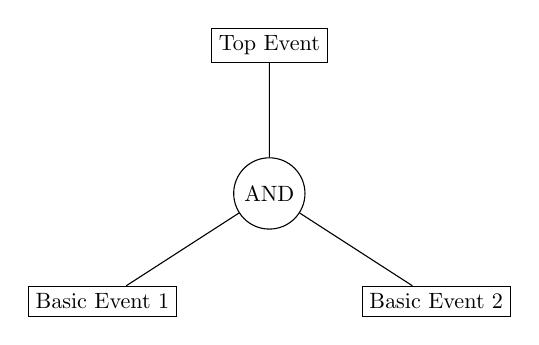
\begin{tikzpicture}[node distance=1.5cm, scale=0.8, transform shape]
\node (top) [rectangle, draw] {Top Event};
\node (and1) [circle, draw, below=of top] {AND};
\node (basic1) [rectangle, draw, below left=of and1] {Basic Event 1};
\node (basic2) [rectangle, draw, below right=of and1] {Basic Event 2};
\draw [-] (basic1) -- (and1);
\draw [-] (basic2) -- (and1);
\draw [-] (and1) -- (top);
\end{tikzpicture}
\end{minipage}%
\hfill % Fills the space between minipages
\begin{minipage}[t]{0.48\textwidth}
\centering
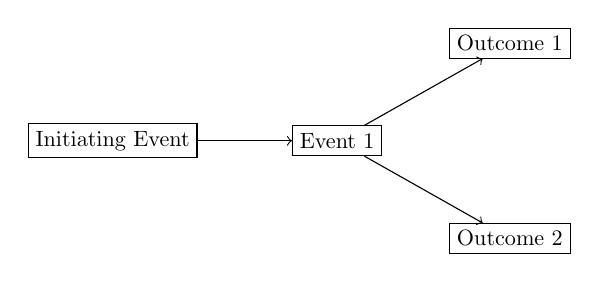
\begin{tikzpicture}[node distance=1.5cm, scale=0.8, transform shape, auto]
\node (init) [rectangle, draw] {Initiating Event};
\node (event1) [rectangle, draw, right=of init] {Event 1};
\node (outcome1) [rectangle, draw, above right=of event1] {Outcome 1};
\node (outcome2) [rectangle, draw, below right=of event1] {Outcome 2};
\draw [->] (init) -- (event1);
\draw [->] (event1) -- (outcome1);
\draw [->] (event1) -- (outcome2);
\end{tikzpicture}
\end{minipage}
\newline
\bottomrule

\newpage \subsubsection*{Did you know? - Bowtie Model}
\begin{mdframed}[backgroundcolor=gray!20] 
Bowtie Model in Risk Management: The bowtie model, which combines elements of both FTA and ETA, provides a visually intuitive way to understand and manage risks. By linking causes to effects through a central event, the model offers a holistic view of risk management strategies, emphasizing the importance of both prevention and mitigation.
\end{mdframed}

\subsection*{Cut Sets and Path Sets}
In the realm of Probability Assessment, particularly within the methodologies of Fault Tree Analysis (FTA) and Event Tree Analysis (ETA), the concepts of Cut Sets and Path Sets play crucial roles. These sets help in dissecting the system's reliability structure, offering insights into how component failures can lead to system-wide impacts or how certain components ensure system functionality. 

\subsubsection*{Cut set}
    \begin{itemize}
        \item Description: A combination of component failures that would lead to system failure.
        \item Importance: Identifying cut sets helps in understanding how different failures can combine to cause system failure.
        \item \textbf{Minimum Cut Set} The smallest set of failures that can cause system failure. It is useful for prioritizing which components to make more reliable to improve overall system safety.
    \end{itemize}
\subsubsection*{Path Set}
    \begin{itemize}
        \item Description: A set of components that, if operational, ensure the system's success.
        \item Application: Used to identify critical paths in a system for maintaining functionality.
        \item \textbf{Minimum Path Set}The smallest set of operational components necessary for system success. It helps in focusing on essential components for system reliability.
    \end{itemize}

\subsection*{Risk Estimation and Evaluation}
With hazards identified and their probabilities assessed, the next step involves estimating and evaluating the overall risk:

\begin{itemize}
    \item \textbf{Risk Estimation}: Calculates the frequency and severity of hazardous events.
    \item \textbf{Risk Evaluation}: Compares the estimated risks against predefined criteria to ascertain their acceptability or necessitate mitigation.
\end{itemize}

\subsection*{Risk Management}
The final step in the QRA process is risk management. This phase involves developing and implementing strategies to mitigate identified risks, as well as monitoring and reviewing the effectiveness of these strategies over time. Effective risk management not only aims to reduce the likelihood and impact of hazardous events but also ensures that the system remains robust against future risks.

\begin{itemize}
    \item \textbf{Risk Mitigation Strategies}: Develops and executes plans to reduce or eliminate risks.
    \item \textbf{Monitoring and Review}: Involves ongoing surveillance of the risk landscape and reassessment of risk management efficacy.
\end{itemize}


\end{document}
